\subsection{AVL-Trees}

\begin{frame}{Balanced Trees}{AVL-Tree}
  \textbf{AVL-Tree:}
  \begin{itemize}
    \item
      Search tree with modified \texttt{\color{Mittel-Blau}insert} and
      \texttt{\color{Mittel-Blau}remove} operations optimize the
      {\color{Mittel-Blau}depth} of the tree
    \item
      Prevents degeneration of the search tree
    \item
      Height difference of left and right subtree is at maximum one
    \item
      With that the height of the search tree is always
      ${\color{Mittel-Blau}\mathcal{O}(\log n)}$
    \item
      We can perform all basic operations in
      ${\color{Mittel-Blau}\mathcal{O}(\log n)}$
  \end{itemize}
\end{frame}

%-------------------------------------------------------------------------------

\begin{frame}{Balanced Trees}{AVL-Tree}
  \begin{figure}
    \begin{adjustbox}{width=0.75\linewidth}
      \begin{tikzpicture}[
  node/.style={
    circle,
    draw=black,
    color=black,
    line width=0.1em,
    minimum size=2.0em,
    inner sep=0em
  }, path/.style={
    line width=0.25em,
    color=Mittel-Blau
  }, path_error/.style={
    line width=0.25em,
    color=red
  }, lleft/.style={
    color=Mittel-Gruen,
    shift={(-1.0em,-0.75em)}
  }, lright/.style={
    color=Mittel-Gruen!80!black,
    shift={(1.0em,-0.75em)}
  }, level/.style={
    sibling distance = 16.0em/#1,
    level distance = 4.0em
  }, level 3/.style={
    sibling distance = 3.5em,
  }]
\node (0, 0) [node, label={[lleft]:0}] (root) {8}
child [->, path] {
  node [node, label={[lleft]:0}] {4}
  child [->, path] {
    node [node, label={[lleft]:0}] {2}
    child [->, path] { node [node, label={[lleft]:0}] {1} }
    child [->, path] { node [node, label={[lright]:0}] {3} }
  }
  child [->, path] {
    node [node, label={[lright]:0}] {6}
    child [->, path] { node [node, label={[lleft]:0}] {5} }
    child [->, path] { node [node, label={[lright]:0}] {7} }
  }
}
child [->, path] {
  node [node, label={[lright]:0}] {12}
  child [->, path] {
    node [node, label={[lleft]:0}] {10}
    child [->, path] { node [node, label={[lleft]:0}] {9} }
    child [->, path] { node [node, label={[lright]:0}] {11} }
  }
  child [->, path] {
    node [node, label={[lright]:0}] {14}
    child [->, path] { node [node, label={[lleft]:0}] {13} }
    child [->, path] { node [node, label={[lright]:0}] {15} }
  }
};
\end{tikzpicture}
    \end{adjustbox}
    \caption{Example of an AVL-Tree}
    \label{fig:balanced_trees:avl_tree_example1}
  \end{figure}
\end{frame}

%-------------------------------------------------------------------------------

\begin{frame}{Balanced Trees}{AVL-Tree}
  \begin{figure}
    \begin{adjustbox}{width=0.75\linewidth}
      \begin{tikzpicture}[
  node/.style={
    circle,
    draw=black,
    color=black,
    line width=0.1em,
    minimum size=2.0em,
    inner sep=0em
  }, path/.style={
    line width=0.25em,
    color=Mittel-Blau
  }, path_error/.style={
    line width=0.25em,
    color=red
  }, lleft/.style={
    color=Mittel-Gruen,
    shift={(-1.0em,-0.75em)}
  }, lright/.style={
    color=Mittel-Gruen!80!black,
    shift={(1.0em,-0.75em)}
  }, level/.style={
    sibling distance = 16.0em/#1,
    level distance = 4.0em
  }, level 3/.style={
    sibling distance = 3.5em,
  }]
\node (0, 0) [node, label={[lleft, shift={(-0.25em,0.0em)}]:-2}] (root) {8}
child [->, path] {
  node [node, label={[lleft]:0}] {4}
  child [->, path] {
    node [node, label={[lleft]:0}] {2}
    child [->, path] { node [node, label={[lleft]:0}] {1} }
    child [->, path] { node [node, label={[lright]:0}] {3} }
  }
  child [->, path] {
    node [node, label={[lright]:0}] {6}
    child [->, path] { node [node, label={[lleft]:0}] {5} }
    child [->, path] { node [node, label={[lright]:0}] {7} }
  }
}
child [->, path] {
  node [node, label={[lright]:0}] {14}
};
\end{tikzpicture}
    \end{adjustbox}
    \caption{\textbf{Not} an AVL-Tree}
    \label{fig:balanced_trees:avl_tree_example2}
  \end{figure}
\end{frame}

%-------------------------------------------------------------------------------

\begin{frame}{Balanced Trees}{AVL-Tree}
  \begin{figure}
    \begin{adjustbox}{width=0.75\linewidth}
      \begin{tikzpicture}[
  node/.style={
    circle,
    draw=black,
    color=black,
    line width=0.1em,
    minimum size=2.0em,
    inner sep=0em
  }, path/.style={
    line width=0.25em,
    color=Mittel-Blau
  }, path_error/.style={
    line width=0.25em,
    color=red
  }, lleft/.style={
    color=Mittel-Gruen,
    shift={(-1.0em,-0.75em)}
  }, lright/.style={
    color=Mittel-Gruen!80!black,
    shift={(1.0em,-0.75em)}
  }, level/.style={
    sibling distance = 16.0em/#1,
    level distance = 4.0em
  }, level 3/.style={
    sibling distance = 3.5em,
  }]
\node (0, 0) [node, label={[lleft, shift={(-0.25em,0.0em)}]:-1}] (root) {17}
child [->, path] {
  node [node, label={[lleft]:0}] {5}
  child [->, path] {
    node [node, label={[lleft]:0}] {3}
    child [->, path] { node [node, label={[lleft]:0}] {2} }
    child [->, path] { node [node, label={[lright]:0}] {4} }
  }
  child [->, path] {
    node [node, label={[lright, shift={(0.25em,0.0em)}]:-1}] {8}
    child [->, path] { node [node, label={[lleft]:0}] {6} }
  }
}
child [->, path] {
  node [node, label={[lright]:0}] {47}
  child [->, path] {
    node [node, label={[lleft]:0}] {43}
  }
  child [->, path] {
    node [node, label={[lright]:0}] {60}
  }
};
\end{tikzpicture}
    \end{adjustbox}
    \caption{Another example of an AVL-Tree}
    \label{fig:balanced_trees:avl_tree_example3}
  \end{figure}
\end{frame}

%-------------------------------------------------------------------------------

\begin{frame}{Balanced Trees}{AVL-Tree - Rebalancing}
  \textbf{Rotation:}
  \begin{itemize}
    \item
      Central operation of {\color{Mittel-Blau}rebalancing}
    \item
      After rotation:
      \begin{itemize}
        \item
          Subtree {\color{Mittel-Blau}$A$} is a layer higher and subtree
          {\color{Mittel-Blau}$C$} a layer lower
        \item
          The parent child ralation between nodes {\color{Mittel-Blau}$x$} and
          {\color{Mittel-Blau}$y$} have been swapped
      \end{itemize}
  \end{itemize}
  \vspace{-2.5em}
  \begin{columns}
    \begin{column}{0.35\linewidth}
      \begin{figure}
        \begin{adjustbox}{width=\linewidth}
          \begin{tikzpicture}[
  root/.style={
    draw=none
  }, node/.style={
    rectangle,
    color=black,
    draw=Mittel-Blau,
    fill=Hell-Blau,
    line width=0.15em,
    minimum size=2.0em,
    inner sep=0em
  }, path_start/.style={
%    -{Computer Modern Rightarrow[length=0.5em]},
    -{Stealth[length=1.25em]},
    line width=0.25em,
    color=Mittel-Gruen
  }, path/.style={
    path_start,
%    {Circle[scale=0.5,round]}-{Computer Modern Rightarrow[length=0.5em]},
    {Circle[scale=0.5,round]}-{Stealth[length=1.25em]},
    shorten <=-0.35em
  }, tree/.style={
    draw,
    very thick,
    shape border uses incircle,
    shape border rotate=90,
    isosceles triangle,
    isosceles triangle apex angle=55,
    minimum height=5.0em,
    yshift=-2.5em,
    color=black,
    draw=Mittel-Blau,
    fill=Hell-Blau,
    line width=0.15em
  }, level/.style={
    sibling distance = 2.0em,
  }, level/.style={
    level distance = 3.0em
  }, level 2/.style={
    sibling distance = 8.0em,
    level distance = 5.0em
  }, level 3/.style={
    sibling distance = 8.0em,
    level distance = 5.0em
  }]
\node (0, 0) [root] (root) {}
child [path_start] {
  node [node] {\Large y}
  child [path, edge from parent path={
    (\tikzparentnode.south west) -- (\tikzchildnode.north)}
  ] {
    node [node] {\Large x}
    child [path, edge from parent path={
      (\tikzparentnode.south west) -- (\tikzchildnode.north)}
    ] { node [tree] {\Large A} }
    child [path, edge from parent path={
      (\tikzparentnode.south east) -- (\tikzchildnode.north)}
    ] { node [tree] {\Large B} }
  }
  child [path, edge from parent path={
    (\tikzparentnode.south east) -- (\tikzchildnode.north)}
  ] { node [tree] {\Large C} }
};
\end{tikzpicture}
        \end{adjustbox}
        \vspace{-2.0em}
        \caption{Before rotating}
        \label{fig:balanced_trees:avl_tree_rotate_1}
      \end{figure}
    \end{column}
    \begin{column}{0.1\linewidth}
      \begin{center}
        $\Rightarrow$
      \end{center}
    \end{column}
    \begin{column}{0.35\linewidth}
      \begin{figure}
        \begin{adjustbox}{width=\linewidth}
          \begin{tikzpicture}[
  root/.style={
    draw=none
  }, node/.style={
    rectangle,
    color=black,
    draw=Mittel-Blau,
    fill=Hell-Blau,
    line width=0.15em,
    minimum size=2.0em,
    inner sep=0em
  }, path_start/.style={
%    -{Computer Modern Rightarrow[length=0.5em]},
    -{Stealth[length=1.25em]},
    line width=0.25em,
    color=Mittel-Gruen
  }, path/.style={
    path_start,
%    {Circle[scale=0.5,round]}-{Computer Modern Rightarrow[length=0.5em]},
    {Circle[scale=0.5,round]}-{Stealth[length=1.25em]},
    shorten <=-0.35em
  }, tree/.style={
    draw,
    very thick,
    shape border uses incircle,
    shape border rotate=90,
    isosceles triangle,
    isosceles triangle apex angle=55,
    minimum height=5.0em,
    yshift=-2.5em,
    color=black,
    draw=Mittel-Blau,
    fill=Hell-Blau,
    line width=0.15em
  }, level/.style={
    sibling distance = 2.0em,
  }, level/.style={
    level distance = 3.0em
  }, level 2/.style={
    sibling distance = 8.0em,
    level distance = 5.0em
  }, level 3/.style={
    sibling distance = 8.0em,
    level distance = 5.0em
  }]
\node (0, 0) [root] (root) {}
child [path_start] {
  node [node] {\Large x}
  child [path, edge from parent path={
    (\tikzparentnode.south west) -- (\tikzchildnode.north)}
  ] { node [tree] {\Large A} }
  child [path, edge from parent path={
    (\tikzparentnode.south east) -- (\tikzchildnode.north)}
  ] {
    node [node] {\Large y}
    child [path, edge from parent path={
      (\tikzparentnode.south west) -- (\tikzchildnode.north)}
    ] { node [tree] {\Large B} }
    child [path, edge from parent path={
      (\tikzparentnode.south east) -- (\tikzchildnode.north)}
    ] { node [tree] {\Large C} }
  }
};
\end{tikzpicture}
        \end{adjustbox}
        \vspace{-2.0em}
        \caption{After rotating}
        \label{fig:balanced_trees:avl_tree_rotate_2}
      \end{figure}
    \end{column}
  \end{columns}
\end{frame}

%-------------------------------------------------------------------------------

\begin{frame}{Balanced Trees}{AVL-Tree - Rebalancing}
  \textbf{AVL-Tree:}
  \begin{itemize}
    \item
      If a height difference of $\pm 2$ occurs on an
      \texttt{\color{Mittel-Blau}insert} or
      \texttt{\color{Mittel-Blau}remove} operation the tree is rebalanced
    \item
      Many different cases of rebalancing
    \item
      \textbf{Example:}
      \texttt{\color{Mittel-Blau}insert} of $1,2,3,\dotsc$
  \end{itemize}
  \begin{figure}
    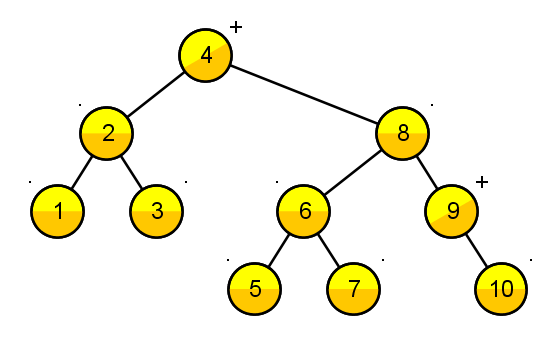
\includegraphics[width=0.5\linewidth]
      {Lecture/Images/AVL-Tree/AVL-Tree_Insert1To10.png}
    \caption{Inserting $1,\dots,10$ into an AVL-tree~\cite{gnarley_trees}}
    \label{fig:balanced_trees:avl_tree_example4}
  \end{figure}
\end{frame}

%-------------------------------------------------------------------------------

\begin{frame}{Balanced Trees}{AVL-Tree - Summary}
  \textbf{Summary:}
  \begin{itemize}
    \item
      Historical the first search tree providing guaranteed
      \texttt{\color{Mittel-Blau}insert}, \texttt{\color{Mittel-Blau}remove}
      and \texttt{\color{Mittel-Blau}lookup} in
      ${\color{Mittel-Blau}\mathcal{O}(\log n)}$
    \item
      Not amortized update costs of $\mathcal{O}(1)$
    \item
      Additional memory costs:
      We have to save a height difference for every node
    \item
      Better (and easier) to implement are {\color{Mittel-Blau}(a,b)}-trees
  \end{itemize}
\end{frame}